\documentclass[11pt]{article}

\usepackage[left=3cm,top=2cm,bottom=2cm,right=3cm]{geometry}
\usepackage{amsmath}
\usepackage{amsfonts}
\usepackage{algorithm}
\usepackage{algorithmic}
\usepackage{array}
\usepackage{graphicx}
\usepackage{subfigure}
\usepackage{epsf}
\usepackage{psfrag}
\usepackage{epsfig}
\usepackage{textcomp}
% \usepackage{hyperref}
\PassOptionsToPackage{hyphens}{url}\usepackage{hyperref}
\usepackage[dvipsnames]{xcolor}
\newcommand{\comment}[1]{{}}

\newcommand{\hwproblem}[2] {\noindent \\ {\bf #1} {\it #2}}

\newcommand{\textbox}[1]{\hfill\rule{0ex}{0.01ex}
 \centerline{\fbox{\parbox{\textwidth}{#1}}}}


\pagestyle{plain} % Header is clear and the footer contains the page number
\setlength{\parindent}{0pt}
\addtolength{\parskip}{\baselineskip}


\begin{document}


% Header
\begin{center}
\small{MIT CSAIL} \\
\vspace{0.1cm}
\large{6.8300/6.8301 Advances in Computer Vision} \\
\vspace{0.2cm}
Spring 2024\\
\vspace{1cm}
{\bf Problem Set 5}
\vspace{0.2cm}
\end{center}

% Administration
\textbox{
\textbf{Posted:} Tuesday, March 19, 2024  \hfill  \textbf{Due:} Tuesday 11:59 pm, April 2, 2024\\

\textbf{Gradescope Instructions:} This week, (1) convert your completed .ipynb notebook to .pdf and submit.  (2) Also submit a .ipynb submission to a second portal.\\

We have provided a helper notebook to help automate .ipynb to .pdf in Colab. \textbf{Make sure your conversion to PDF includes your correct answers,} since sometimes the conversion cuts off answers. \textbf{Overlong programming lines might get cut off.} If you want to write comments, add markdown text boxes with prominent headers. Please note that 6.8301 students will not receive credit for problems which are only for 6.8300. \\

\textbf{Attention:} Unreported work gets a zero: please run all cells first. \\

\textbf{Attention:} Only one file per submission portal. No .zip.\\

\textbf{Late Submission Policy:} If your problem set is submitted within a week of the original deadline, you will receive partial credit. Such submissions will be penalized by a multiplicative coefficient that decreases from 1 to 0.5, daily stepwise.}\\
\vspace{0.2cm}


The aim of this problem set is to study some common issues that may appear when developing a clinical decision support model. We will use the CBIS-DDSM/DDSM dataset, which is a database of scanned film mammography images. It contains normal, benign, and malignant cases\footnote{\url{https://wiki.cancerimagingarchive.net/display/Public/CBIS-DDSM}}. You will train a simple model to classify these images, learn to evaluate the model using different metrics, and analyze some of the problems that arise when using these systems in practice. 
% This Pset is not a comprehensive summary of the potential sources of bias/harm, and the problems studied are heavily simplified so that they can be studied concisely. However, we hope that this pset and the references provided will give you a start to delve deeper into this important set of topics. 

\hwproblem{Problem 1}{Train an Image Classifier (20 points) }

You will use the experience you gained in Pset 4 to train a simple image model that learns to produce a diagnosis in the categories: normal, malignant and benign. Experiment with some of the hyperparameters, techniques, and model types that are proposed in the notebook. 

List the final model type, set of techniques, and hyperparameters you choose (e.g., ResNet-18, data augmentation by rotation, SGD optimizer, learning rate of 0.5, $10\%$ dropout) and explain how they affect model performance (theoretically or intuitively). Report the train, validation, and test top-1 accuracy of your final network. Your trained network should achieve a test accuracy of at least $90\%$ to get a full score on the problem. 


For the rest of the problem set, you can either use your model or the one trained by the instructors (which is automatically downloaded in the notebook). If the test performance of your own model is less than 93\%, please use the latter. 

\hwproblem{Problem 2}{ Metrics (20 points)}

In the previous question, you may have achieved high accuracy, but that doesn't necessarily mean that the model is useful for clinic decision support in practice. Suppose that your model just learns nothing and outputs ``normal'' for every image. If 90\% of the patient images in your dataset are normal, the accuracy is still as high as 90\%! In this question, we will introduce some other metrics commonly used when your dataset is imbalanced, as in biomedical imaging tasks. \textbf{For a better understanding of these metrics, please don't use pre-defined functions for these metrics from other libraries.} 

\textbf{(a) Confusion Matrix}

Classification accuracy alone can hide important details if you have an unequal number of observations in each class or if you have more than two classes in your dataset. A confusion matrix helps you summarize the performance of a classification algorithm and can give you a better idea of what your classification model is getting right and what types of errors it is making. 

In the provided notebook, \textbf{build the function} \texttt{plot\_confusion\_matrix()} \textbf{to plot a confusion matrix for your selected model}. Your confusion matrix should approximately follow the template given in Figure \ref{fig:cm_plot}, but the format doesn't need to match exactly. \textbf{Don't use helper libraries to compute the numbers,} though confusion matrix helper functions for visualization are great. 

\begin{figure}[htp!]
\centering
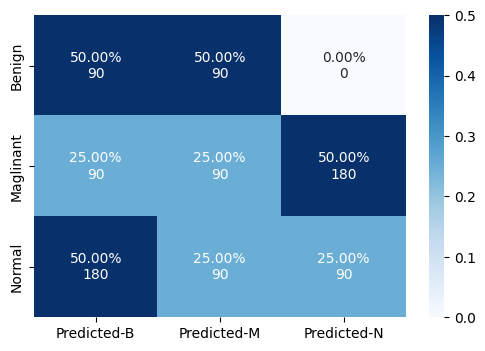
\includegraphics[width = 10cm]{cm_template.png}
\caption{Confusion Matrix Template}
\label{fig:cm_plot}
\end{figure}

\textbf{(b) Precision-Recall Curve}

A precision recall curve is a 2D plot showing precision and recall values for different decision thresholds in a binary classification problem. Typically, the decision threshold is 0.5: if the predicted probability of class A is, say, 0.7, then the probability of class B will be 0.3 (they always sum to 1), and we choose class A as our predicted class.

For those classification problems that have a severe class imbalance, the default threshold can result in poor performance. As such, a simple and straightforward approach to improving the performance of a classifier that predicts probabilities on an imbalanced classification problem is to tune the threshold used to map probabilities to class labels.

Our dataset has 3 classes and in order to be able to compute metrics commonly used in binary classification, you need to create binary labels from the given class labels. We will assume a scenario where we really care about malignant cases. \textbf{Please consider the malignant class (label 1) as the positive class and consider the benign (label 0) and normal (label 2) classes together as the negative class.}

In this scenario, if we use the default threshold of 0.5, and our classifier predicts a 0.6 for class malignant, 0.3 for class benign and 0.1 for class normal (always sums to 1!), we would confidently assign a positive class to that example. If we change our threshold to 0.7, however, we will assume that our example is part of the \textit{negative class} for the purposes of calculating precision and recall.

Before proceeding, please familiarize yourself with the following terms commonly used in binary classification: True Positive (TP), True Negative (TN), False Positive (FP), and False Negative (FN). Here, we are interested in two combinations of these quantities: Precision (P = TP/(TP+FP)) and Recall (R = TP/(TP+FN)). 

Which one should you look at when you are trying to improve the model? It really depends on the problem at hand. For example, if you are trying to detect people with allergies, you don't want to alert too many people who may not have allergies (FP) and therefore you want a high precision. However, in cases such as cancer prevention, a false negative is usually more disastrous than a false positive so you want a high recall. You could have 100\% recall by predicting the positive class for everyone but then you would have a completely uninformative model. This is where the precision-recall curve can be helpful in balancing the trade-off between precision and recall by using different probability cutoffs, or thresholds.

As we indicated above, the malignant class is our positive class, and the rest are negative classes. In this scenario, a positive prediction happens when our model's prediction for class malignant is above a user-defined threshold. That means that a True Positive happens when we have a positive prediction, and the ground truth label is malignant. A False Positive happens when we have a positive prediction and the ground truth label is something other than malignant. True negatives and false negatives follow the same logic.

 \textbf{In the provided notebook, calculate precision and recall for 1000 evenly spaced thresholds between 0 and 1, and plot the precision-recall curve of your selected model. Then, compute the AUC leveraging the function \texttt{trapz} from numpy, and display the AUC on the plot.} Your output for this question should be one plot, with precision on the Y axis and recall on the X axis.

\hwproblem{Problem 3}{What is the model looking at? (10 points)}

A common technique used to delve deeper into trained models is visualizations. As studied in the previous problem set, filter visualizations are sometimes useful to understand how the network behaves, but it is hard for non-expert users to interpret them.

Another technique previously studied is CAM visualizations, which provide a simple way to interpret what regions of the image contribute to the prediction for each output target. This is a useful tool to check whether the model is picking up spurious correlations or the predictions focus on regions of the image that are consistent with expert knowledge. 
Run Grad-CAM (or another CAM visualization) on several images for the different test sets, and explain the differences you see between correctly and incorrectly classified samples.


\hwproblem{Problem 4}{Evaluation on an External Dataset (6.8301: 20 points, 6.8300: 30 points)}

In this question, we will study a problem that occurs frequently in practice when deploying systems. Oftentimes, the data distribution at test time is different from the one used during training.

(a) (10 points) To begin, visually compare the performance with the original model against an external dataset of the same type, provided in \texttt{external\_dataset\_dir}.

(b) (10 points) Compare samples of the two datasets visually, and report the differences that you observe. (Hint: if you need inspiration, check typical image transformations in PyTorch under \texttt{torchvision.transforms}.)

(c) (10 points)  {\bf [6.8300 only]} Implement a set of transformations that can be applied to the original dataset at train time that would mitigate this issue. Plot the original dataset with the proposed transformations, which should produce qualitatively similar samples as the external dataset. Although you don't need to retrain the model, you are free to do so to further check that the transformations are correct (performance on the external dataset should improve using the original data with the extra transformations). Use some of the available PyTorch transformations under \texttt{torchvision.transforms}.

\hwproblem{Problem 5}{Class Imbalance (6.8301: 20 points, 6.8300: 40 points)}

An issue typically present in medical datasets is class imbalance: patients that do not have the disease are more frequent than patients that do have the disease. One way to make the trained model perform differently is by simulating a dataset that contains a different number of samples of each category. This can be achieved by at least two methods: reweighting the loss and changing the sampling procedure.

(a) Implement reweighting of the loss so that all classes contribute equally to the loss. 

(b) Modify the dataset so that samples for the three classes are balanced. 

(c) {\bf [6.8300 only]} Finally, train your original model with the two modifications, plot the confusion matrix for them, and answer the following questions:

\begin{itemize}
 \item What are the empirical differences you see (if any) between the two approaches for addressing class imbalance?
\item What are the theoretical differences between the two techniques? 
\item What are the strengths and weaknesses of the techniques?
\end{itemize}

Hint: think about gradient estimation in the extreme case where the number of samples of the less predominant class is low. 

\hwproblem{Reading list}

\begin{itemize}
    \item Understanding Potential Sources of Harm throughout the Machine Learning Life Cycle by Harini Suresh and John Guttag. (\url{https://mit-serc.pubpub.org/pub/potential-sources-of-harm-throughout-the-machine-learning-life-cycle/release/1})
\end{itemize}
% \bibliographystyle{plain}
% \bibliography{pset5}
\end{document}